\subsection{Aplicação Fábrica: Produção}
\subsubsection*{Descrição do caso de uso}
No registo de produção, espera-se que utilizador entre na página e indique o código de barras da recolha, o peso de cera, metal e plástico e o seu ID. A informação da data de produção deve ser indicada automaticamente pelo sistema e a informação sobre a recolha (ponto de recolha e data da recolha) seja obtido, em background, após indicar o código de barras da recolha.

\begin{figure}[H] 
	\begin{center}
		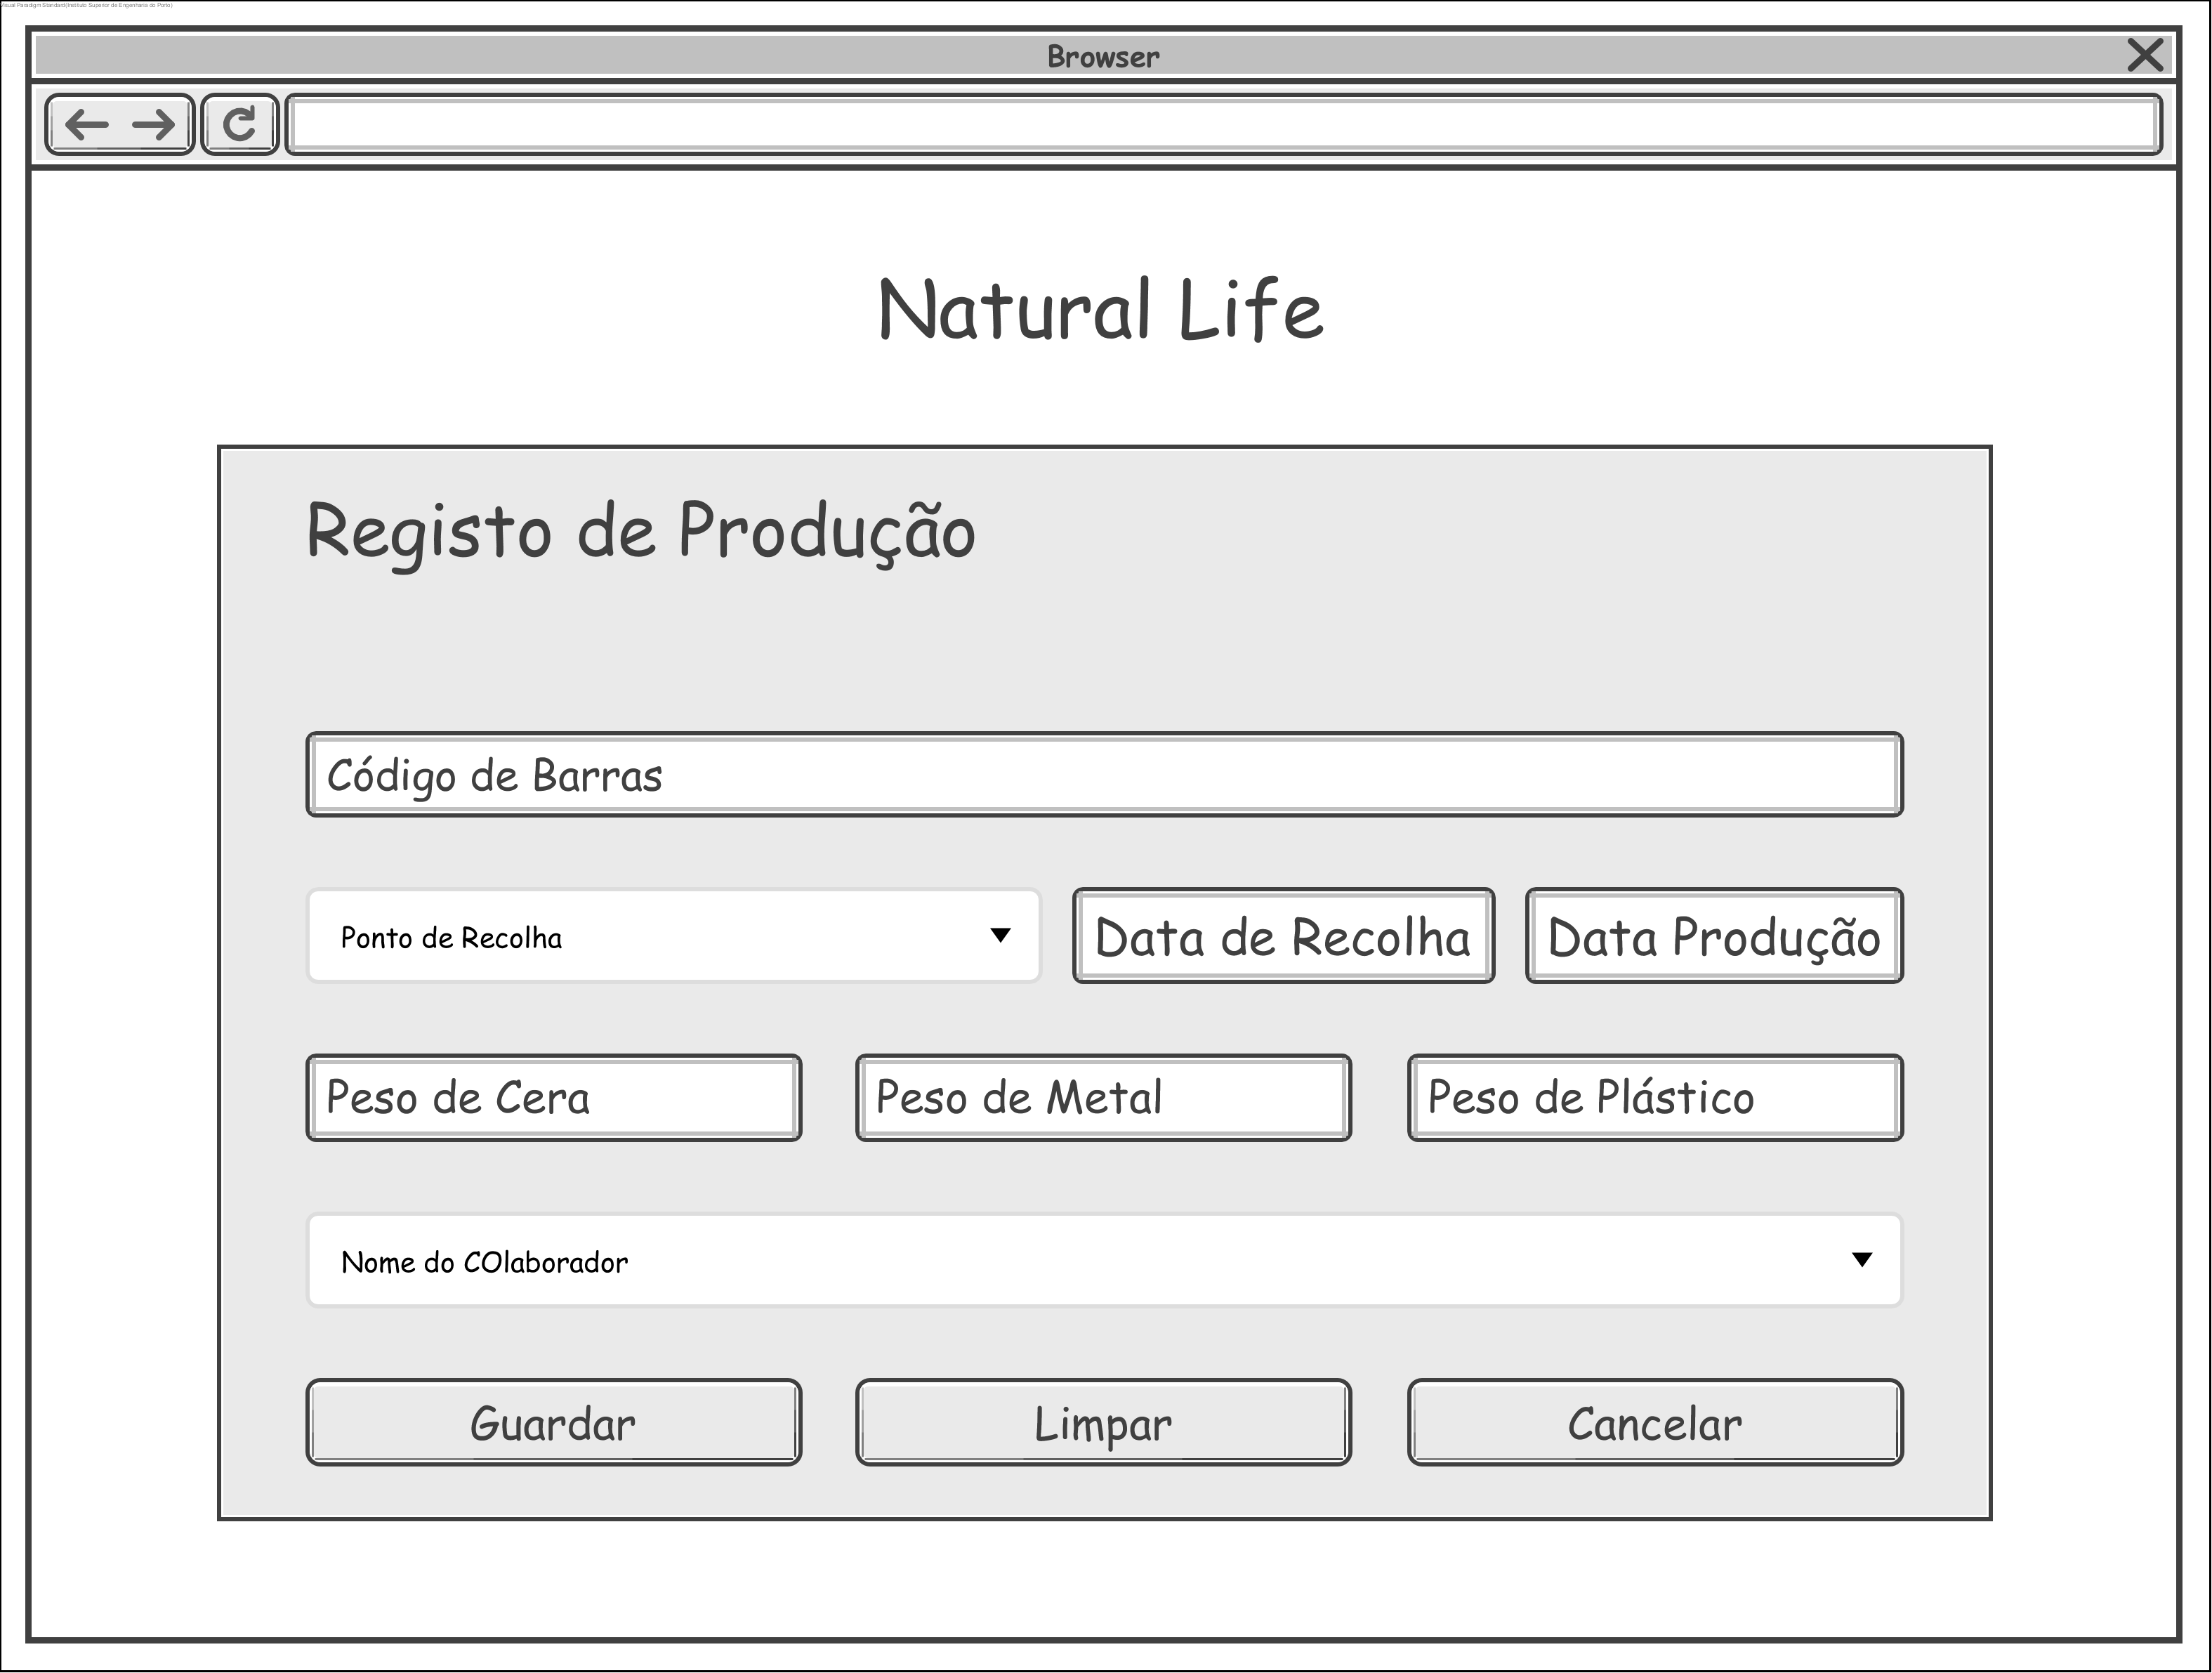
\includegraphics[width=0.60\textwidth,keepaspectratio]{figuras/Diagramas_vp/DI_Fabrica_3-Registo_de_Produção.png}
		\caption{Modelo do formulário do registo de produção}
		\label{fig:di_producao} 
	\end{center}
\end{figure}

\subsubsection*{Fluxo do caso de uso}
O caso de uso inicia-se com a abertura da página do registo de produção. É apresentado o formulário com a data de produção previamente preenchida. O utilizador tem de indicar o código de barras da recolha, peso de cera, metal e plástico e o seu ID numa lista de dropdown. Quando o utilizador termina de indicar o código da recolha é feito um request ao servidor para saber o ponto de recolha e data da recolha. Essa informação é apresentada automaticamente ao utilizador Após indicar as informações solicitadas precisona o botão "Guardar". Após o registo é apresentada uma mensagem ao utilizador.

\begin{figure}[H] 
	\begin{center}
		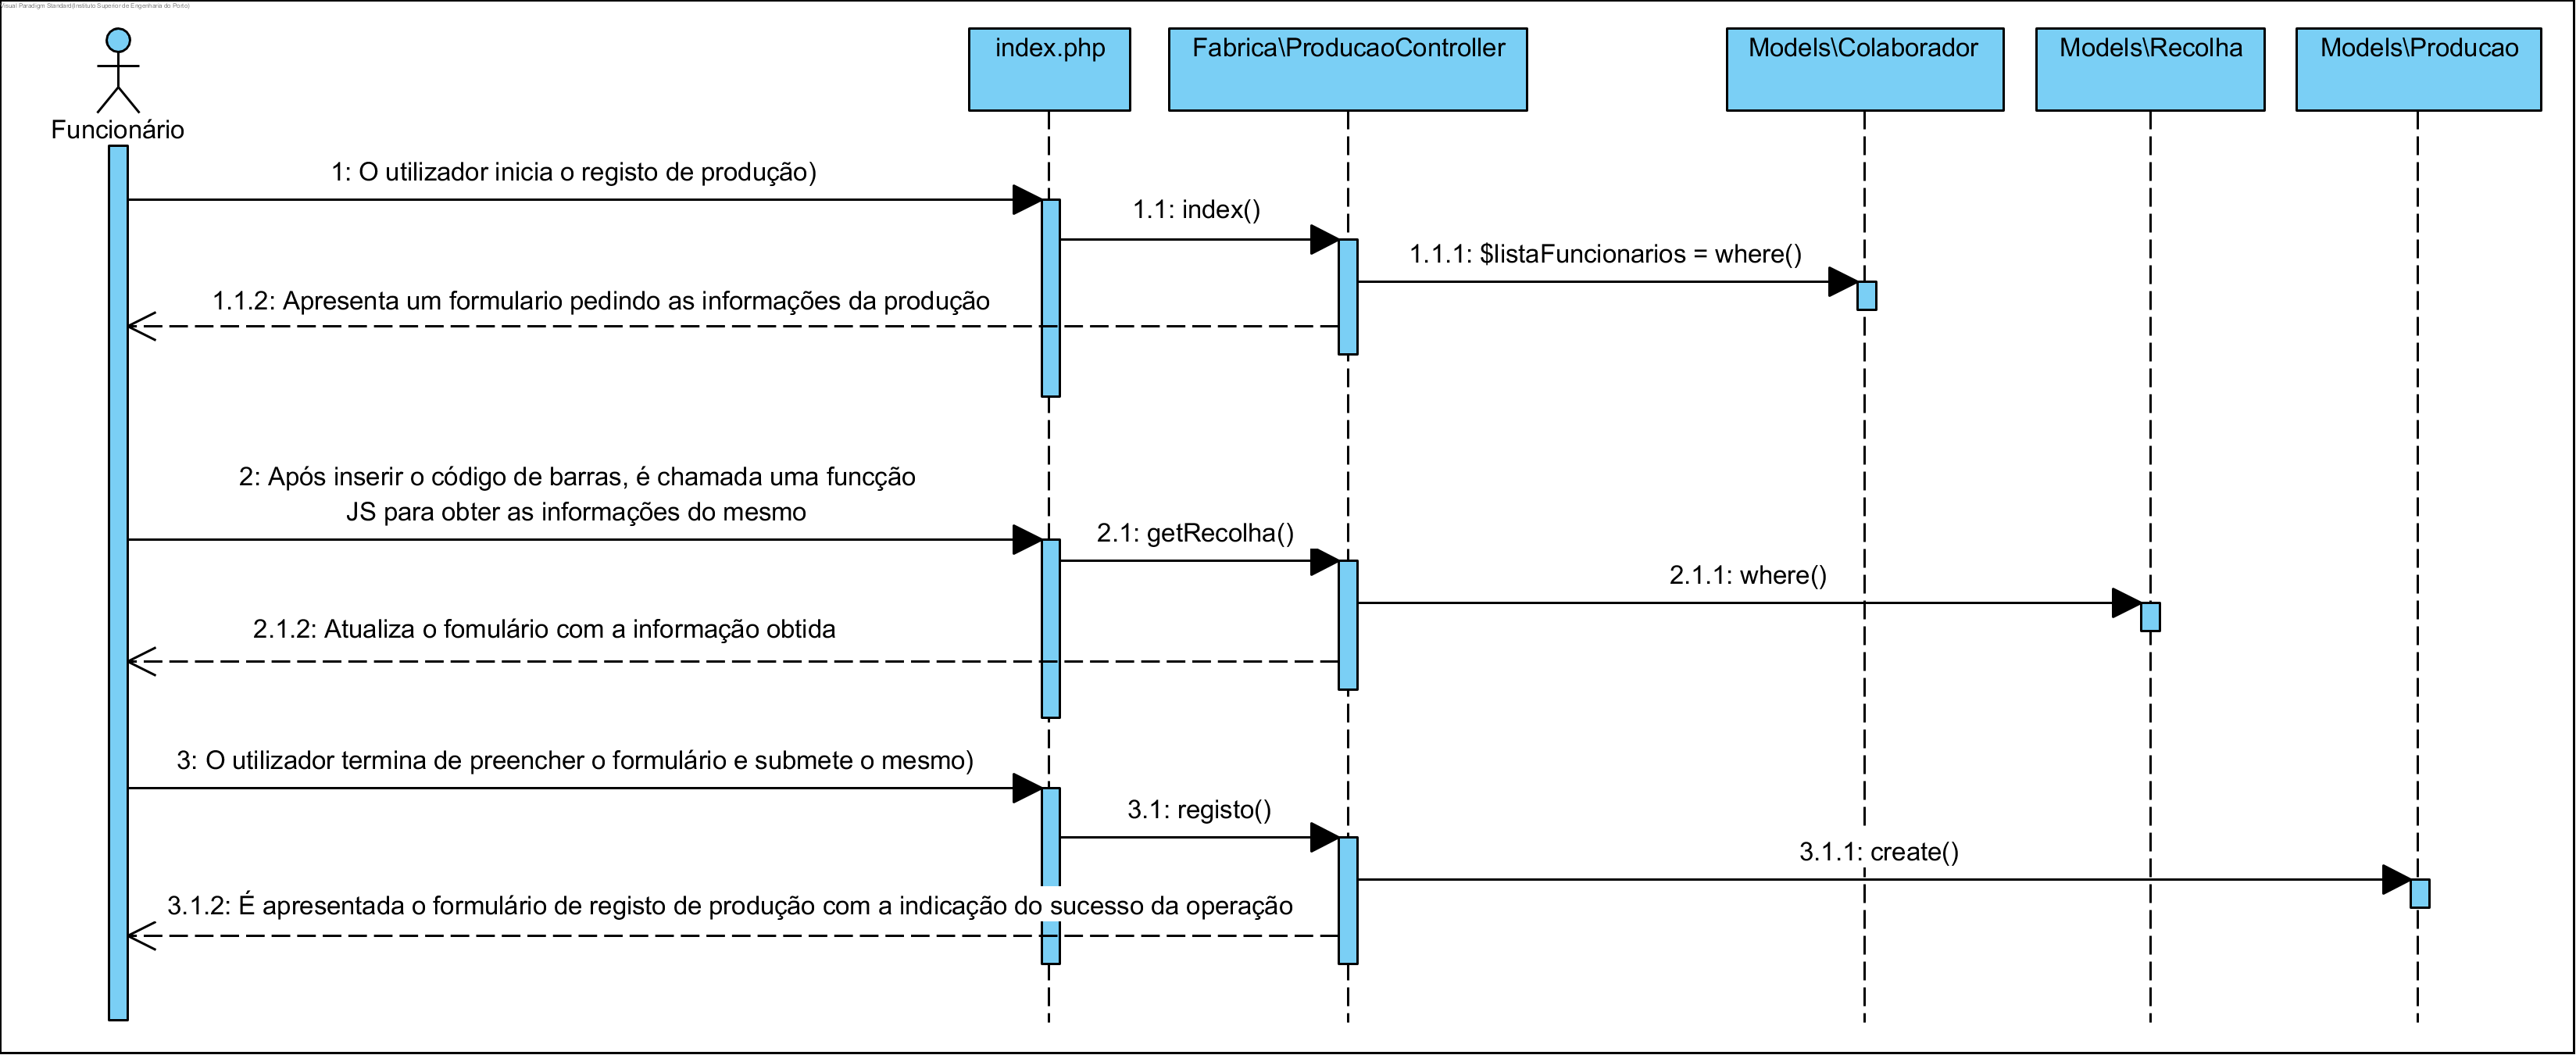
\includegraphics[width=\textwidth,keepaspectratio]{figuras/Diagramas_vp/SD_Fabrica_3-Registo_de_Produção.png}
		\caption{Diagrama de Sequência registo de produção}
		\label{fig:sd_producao} 
	\end{center}
\end{figure}